\documentclass[pdftex,twocolumn,10pt,letterpaper]{extarticle}


%%% Set these variables appropriately
%%%
%% Note:  Authors is hardcoded below, this line only used for the PDF info
\newcommand{\AUTHORS}{authors}
% Title needs work
\newcommand{\TITLE}{something}
\newcommand{\KEYWORDS}{Put your keywords here}
\newcommand{\CONFERENCE}{Somewhere}
\newcommand{\PAGENUMBERS}{yes}       % "yes" or "no"
\newcommand{\COLOR}{yes}
\newcommand{\showComments}{yes}
\newcommand{\comment}[1]{}
\newcommand{\onlyAbstract}{no}

\newcommand{\lv}[1]{\textcolor{red}{(\textbf{LV:#1} )}}


%%%%%%%%%%%%%%%%%%%%%%%%%%%%%%%%%%%%%%%%%%%%%%%%%%%%%%%%%%%%%%%%%%%%%
% ACM Fonts

\newfont{\secfnt}{ptmb8t at 12pt}
\newfont{\secit}{ptmbi8t at 12pt}    %13 Jan 00 gkmt
\newfont{\subsecfnt}{ptmri8t at 11pt}
\newfont{\subsecit}{ptmbi8t at 11pt}  % 
\newfont{\ttlfnt}{phvb8t at 18pt}
\newfont{\ttlit}{phvbo8t at 18pt}    % GM 2/4/2000
\newfont{\subttlfnt}{phvr8t at 14pt}
\newfont{\subttlit}{phvro8t at 14pt} % GM 2/4/2000
\newfont{\subttlbf}{phvb8t at 14pt}  % 13 Jan 00 gkmt
\newfont{\aufnt}{phvr8t at 12pt}
\newfont{\auit}{phvro8t at 12pt}     % GM 2/4/2000
\newfont{\affaddr}{phvr8t at 10pt}
\newfont{\affaddrit}{phvro8t at 10pt} % GM 2/4/2000
\newfont{\eaddfnt}{phvr8t at 12pt}
\newfont{\ixpt}{ptmr8t at 9pt}
\newfont{\confname}{ptmri8t at 8pt}
\newfont{\crnotice}{ptmr8t at 8pt}
\newfont{\ninept}{ptmr8t at 9pt}

%%%%%%%%%%%%%%%%%%%%%%%%%%%%%%%%%%%%%%%%%%%%%%%%%%%%%%%%%%%%%%%%%%%%%%

\hyphenation{off-load-ing}

\renewenvironment{itemize}
{\begin{list}{$\bullet$}{
    \setlength{\labelsep}{4pt}
    \setlength{\labelwidth}{3pt}
    \setlength{\rightmargin}{0pt}
    \setlength{\leftmargin}{0pt}
    \addtolength{\leftmargin}{\labelwidth}
    \addtolength{\leftmargin}{\labelsep}
}}{\end{list}}


%%%%%%%%%%%%%%%%%%%%%%%%%%%%%%%%%%%%%%%%%%%%%%%%%%%%%%%%%%%%%%%%%%%%%

%%%
%%%  Page Setup
%%%
\special{papersize=8.5in,11in}
\setlength{\pdfpagewidth}{8.5in}
\setlength{\pdfpageheight}{11in}

\usepackage{ifthen}
\ifthenelse{\equal{\PAGENUMBERS}{yes}}{%
\usepackage[nohead,
% SIGCOMM?
            left=0.75in,right=0.85in,top=0.75in,
% USENIX
%            left=1.0in,right=1.0in,top=1.0in,
            footskip=0.5in,bottom=1.0in,     % Room for page numbers
            columnsep=0.33in
%            columnsep=0.2in  %SPACE
            ]{geometry}
}{%
\usepackage[noheadfoot,left=0.75in,right=0.85in,top=0.75in,
            footskip=0.5in,bottom=1in,
            columnsep=0.25in
	    ]{geometry}
}

\renewenvironment{itemize}
{\begin{list}{$\bullet$}{
    \setlength{\labelsep}{4pt}
    \setlength{\labelwidth}{3pt}
    \setlength{\rightmargin}{0pt}
    \setlength{\leftmargin}{0pt}
    \addtolength{\leftmargin}{\labelwidth}
    \addtolength{\leftmargin}{\labelsep}
}}{\end{list}}


%%%
%%%  Captions
%%%
%\usepackage[font=bf]{caption}
\usepackage[font=small,format=plain,labelfont=bf,textfont=it,aboveskip=4pt]{caption}

%%  Space between figure and caption (assuming caption
%%  is below figure)
%\usepackage[font=bf,aboveskip=0pt]{caption} % SPACE
%%  Space between caption and body text of document
\addtolength{\textfloatsep}{-7pt} % SPACE

%%%
%%%  Section headings
%%%
%\usepackage{titlesec}
%\titlespacing{\paragraph}{0pt}{*1}{*1}      % SPACE
\usepackage[compact]{titlesec}              % SPACE
%\titleformat{\section}%                     % IEEE/ACM: caps + period
%  {\bf\large\uppercase}{\thesection.\quad}{0pt}{}

%%%
%%%  Lists
%%%
\usepackage{paralist}
\usepackage{enumitem}
\setlist{itemsep=0pt,parsep=0pt}             % more compact lists

\renewcommand{\paragraph}[1]{\vspace*{0.03in}\noindent{\bf #1}}

%%%
%%% Custom Environments
%%%

\usepackage{balance}
\usepackage{subcaption}
\usepackage{amsmath, amssymb,alltt}
\usepackage{url,tabularx,amsmath,amssymb,psfrag,times,multirow,color}
\usepackage{listings}
\usepackage{algorithm}
\usepackage{algorithmic}
\usepackage{times}
\usepackage{ifthen}
\usepackage[color]{changebar}
\usepackage{marginnote}
\usepackage{amsthm}
\usepackage{textcomp}
\usepackage{graphicx}


\renewenvironment{itemize}
{\begin{list}{$\bullet$}{
    \setlength{\labelsep}{4pt}
    \setlength{\labelwidth}{3pt}
    \setlength{\rightmargin}{0pt}
    \setlength{\leftmargin}{0pt}
    \addtolength{\leftmargin}{\labelwidth}
    \addtolength{\leftmargin}{\labelsep}
}}{\end{list}}

\definecolor{steel_blue}{RGB}{70, 130, 180}

\lstset{
basicstyle=\footnotesize\ttfamily\small,
frame=none,
language=Python,
numbers=none,
breaklines=true,
xleftmargin=0pt
}


%\lstdefinelanguage{Pyretic}
%{keywords={>>, >+, +, &, push, if_, elif_, else, pop, match, fwd, modify, set, mod, drop, $\triangleleft$, announce, withdraw}, 
%  sensitive=true, alsoletter={-,>>,+,&,|,_},comment=[l][\footnotesize\sffamily\textbf]{\!}
%}
%
%\lstset{emph={View1, CA, CA-IN, as-path, med, no-prepend},
%  keywordstyle=\color{steel_blue}\textbf}
%\lstset{language=Pyretic}


%%%
%%%  Header / Footer
%%%
\usepackage{fancyhdr}

\renewcommand{\headrulewidth}{0pt}

\ifthenelse{\equal{\PAGENUMBERS}{yes}}{%
  \pagestyle{plain}
}{%
  \pagestyle{empty}
}
\usepackage{lastpage}
%%%
%%%  Bibliography
%%%
%\usepackage{cite}
\usepackage[numbers,sort]{natbib}

%%%
%%%  Footnotes / Endnotes
%%%
\interfootnotelinepenalty=10000  % Split footnotes are annoying

% If you want endnodes, uncomment:
%\usepackage{endnotes}
%\usepackage{drafthead}
%\let\footnote=\endnote

%%%
%%%  Tables
%%%
\usepackage{booktabs}
\usepackage{color}
\usepackage{colortbl}
\usepackage{float}                           % Must appear before hyperref to
                                             % avoid weird PDF compile issues

%%%
%%%  Fonts
%%%
\usepackage{mathptmx}                        % Times/Times-like math symbols
%\usepackage{courier}
\usepackage[scaled=0.92]{helvet}

%%%
%%%  PDF setup
%%%
\usepackage[breaklinks=true,filecolor=black,citecolor=blue,urlcolor=black,linkcolor=blue,colorlinks,
pdfpagelabels,pdfpagelayout=SinglePage, pagebackref=true ]{hyperref}
\renewcommand\UrlFont{\rmfamily\itshape}

\renewcommand*{\backref}[1]{}
\renewcommand*{\backrefalt}[4]{
   \ifcase #1 %
     (Not cited.) %
   \or
     {\small\sffamily (Cited on page~#2.)}%
   \else
     {\small\sffamily (Cited on pages~#2.)}%
   \fi
 }
\renewcommand*{\backrefsep}{, }
\renewcommand*{\backreftwosep}{ and~}
\renewcommand*{\backreflastsep}{ and~}

\hypersetup{%
pdfauthor = {\AUTHORS},
pdftitle = {\TITLE},
pdfsubject = {\CONFERENCE},
pdfkeywords = {\KEYWORDS},
bookmarksopen = {true}
}

%%
%% Figure placeholder macros
%%

\definecolor{placeholderbg}{rgb}{0.85,0.85,0.85}
\newcommand{\placeholder}[1]{%
\fcolorbox{black}{placeholderbg}{\parbox[top][1.5in][c]{0.95\columnwidth}{#1}}}


%%%
%%%  Misc
%%%

%\setlength{\parindent}{0pt}
%\setlength{\parskip}{\baselineskip}

\clubpenalty=10000  % Don't allow orphans
\widowpenalty=10000 % Don't allow widows

%%%
%%%  To appear/appeared in text on title page
%%%
\usepackage[absolute]{textpos}
\newcommand{\ToAppear}{%
\begin{textblock*}{\textwidth}(0.95in,0.4in)
\begin{flushright}
    %\noindent{\fbox{\textsf{Under submission---please do not
    %redistribute.}}}
    %  --OR--
    \noindent{\small To appear in \textit{Proceedings of the XYZ}\\
    \noindent{\small \textit{Conference (XYZ'08)}, City, State, Month 2008}}
    %  --OR--
    %\noindent{\small In \textit{Proceedings of the XYZ}\\
    %\noindent{\small \textit{Conference (XYZ'08)}, City, State, Month 2008}}
\end{flushright}
\end{textblock*}
}

%%%
%%%  Sample ACM Copyright Block
%%%
%\newfloat{acmcr}{b}{acmcr}
%\newcommand{\AcmCopyright}{%
%\begin{acmcr}
%\noindent
%\footnotesize
%\renewcommand{\baselinestretch}{0.75}
%\!\!Permission to make digital or hard copies of all or part of this work
%for personal or classroom use is granted without fee provided that
%copies are not made or distributed for profit or commercial advantage
%and that copies bear this notice and the full citation on the first
%page. Copyrights for components of this work owned by others than ACM
%must be honored. Abstracting with credit is permitted. To copy
%otherwise, or republish, to post on servers or to redistribute to
%lists, requires prior specific permission and/or a fee. Request
%permissions from permissions@acm.org.  \\
%{\em SIGCOMM'14}, August 17--22, 2014, Chicago, IL, USA.\\ 
%Copyright 2014 ACM 978-1-4503-2836-4/14/08 ...\$15.00. \\ 
%\url{http://dx.doi.org/10.1145/2619239.2626300}
%\end{acmcr}
%}

%%%
%%% ACM Categories, etc.
%%%


%%%
%%%  Comments
%%%
\newcommand{\note}[2]{
    \ifthenelse{\equal{\showComments}{yes}}{\textcolor{#1}{#2}}{}
}

%%%%%%%%%%%%%%%%%%%%%%%%%%%%%%%%%%%%%%%%%%%%%%%%%%%%%%%%%%%%%%%%%%%%%%%%%%%%%%%%%%%%%%%%
\newcommand{\xxx}[1]{\note{blue}{#1}}		%use for comments
\newcommand{\sg}[1]{\note{red}{#1 -- SG}}			%use for questions
\newcommand{\todo}[1]{\note{green}{TODO: #1}}		%use for todo
%%%%%%%%%%%%%%%%%%%%%%%%%%%%%%%%%%%%%%%%%%%%%%%%%%%%%%%%%%%%%%%%%%%%%%%%%%%%%%%%%%%%%%%%

%%%
%%% Abbreviations
%%%
\newcommand{\ie}{{\em i.e.}}
\newcommand{\eg}{{\em e.g.}}
\newcommand{\ea}{{\em et al.}}
%\newcommand{\system}{FLANC}
%\newcommand{\name}{FLANC}
\newcommand{\test}{test}
\newcommand{\control}{control}
\newcommand{\fp}{\vspace*{0.02in}\noindent}

%% \newtheoremstyle{tighter}
%%     {3pt}        % Space above
%%     {3pt}        % Space below
%%     {\em}        % Body font
%%     {}           % Indentation
%%     {\bfseries}  % Head font
%%     {:}          % Head punctuation
%%     {.5em}       % Head space
%%     {}           % Custom head spec
%% \theoremstyle{tighter}
%\newtheorem{lesson}{Lesson}
%\newtheorem{constraint}{Constraint}
%\newcommand{\lesson}[1]{\vspace{1em}{\centering\fbox{\parbox{0.95\columnwidth}{\centering\bf Lesson: #1}}}\vspace{1em}}


\newcommand{\supsym}[1]{\raisebox{4pt}{{\footnotesize #1}}}
%\newcommand{\ptn}{\supsym{$\dag$}}
%\newcommand{\aff2}{\supsym{$\diamond$}}
%\newcommand{\aff3}{\supsym{$\star$}}
%\newcommand{\aff4}{\supsym{$\ddag$}}

\newcommand{\remove}[1]{}
\newcommand{\cmstart}{}
\newcommand{\cmend}{}
\newtheorem{axiom}{Axiom}
\newtheorem{theorem}{Theorem}

\date{}
\title{
\textbf{\ttlfnt \TITLE}}
\author{
\aufnt{Paper \#0, \pageref{LastPage} Pages}
%\aufnt{Sarthak Grover\ptn, xxx\aff2, yyy\aff3}\\
%\ptn\affaddr{Princeton University}~~~\et\affaddr{ABC, city}
}
%\date{\normalsize\url{http://projectbismark.net}}


% This needs to be the last thing before \begin{document}
\usepackage{microtype}  % SPACE

%%%%%%%%%%%%%%%%%%%%  START DOCUMENT  %%%%%%%%%%%%%%%%%%%%%%%%
\begin{document}

\maketitle

%\AcmCopyright
%\ToAppear

\thispagestyle{empty}

\begin{sloppypar}
\begin{abstract}

The Federal Communications Commission (FCC) has recently taken major decisions in an attempt to 
regulate broadband in the US, creating disputes between itself and ISP providers.
One such policy was the radical increase of broadband speed benchmark, that motivated both parties
to investigate these regulations from different perspectives. This led to the Commission
publically requesting comments on issues pertaining to ``advanced telecommunication capabilities''
to design future benchmarks based on metrics other than broadband speed.

In this work, we provide a much required input to the FCC's open questions,
supported by our analysis of usage patterns, rather than just the FCC’s speed benchmarks.
We analyse users with high tier access links and motivate
the need of multiple benchmarks based on peak usage of different types
of users. We also show that beyond a certain speed, user behavior is not
significantly impacted by further increases in broadband capacity. Therefore,
motivating the need to define benchmarks based on metrics other than broadband
speed to truly offer ``advanced'' capabilities.

\end{abstract}

\ifthenelse{\equal{\onlyAbstract}{no}}{%

%\vspace*{0.1in}
%\fp {\bf Categories and Subject Descriptors:}
%C.2.1 [Computer-Communication Networks] {\em Network Architecture and
%  Design}: Network Communications
%
%\fp {\bf General Terms:}
%Algorithms, Design, Experimentation
%
%\fp
%{\bf Keywords:}
%home networks; Broadband Utilization; FCC; Comcast

\section{Introduction}\label{sec:introduction}

With the large impact of broadband Internet on our daily lives and its
rapid increase in bandwidth-intensive services, policymakers and service
providers (ISPs) are trying to determine how much bandwidth consumers
need. With the proliferation of high quality video content, and the
recent boom in Internet-enabled consumer device, it is worth
studying---and continually re-evaluating---whether (and how) users
consume the capacity that ISPs offer.  Up to a certain point, users will
exhaust available capacity, and they will also adapt when more capacity
becomes available; this increased demand in turn drives provisioning.
Above certain speeds, however, the typical user no longer exhausts the
available capacity. At what speed does this inflection point occur?  How
do users adapt their demands when an ISP offers faster speed tiers?
Answers to these questions will ultimately help inform policymakers and
ISPs determine how to make investments in infrastructure, and when to
make them.

In the United States, the Federal Communications Commission (FCC) is
interested in the relationship between demand and capacity for several
reasons.  First, the FCC recognizes the need to define broadband
benchmarks based on traffic demand and is considering doing
so~\cite{fcc2015broadband-report}. It has defined a ``typical''
household traffic demand to enable concurrent broadband use, such as
video streaming, web browsing, and VoIP. Currently, the FCC is asking
for comments and suggestions on how to define such a demand-based
benchmark for future planning~\cite{fcc2015progress-report,
  fcc2014progress-report}.  Second, recent research shows that diurnal
Internet usage patterns are correlated with GDP, Internet allocations,
as well as electrical consumption of a
region~\cite{ant-diurnal-web}. This makes the study of usage extremely
relevant to the regulatory bodies responsible for development.  Finally,
the FCC is responsible for increasing broadband deployment throughout
the US, and it recently decided to aggressively increase the broadband
threshold benchmark to 25 Mbps in downlink and 3 Mbps in uplink.  Yet, a
survey conducted by NCTA (for the FCC) showed that the largest deterrent
to deployment of faster speed tiers is that consumers do not \emph{want}
the faster speeds (the second largest deterrent is the
price)~\cite{fcc2015progress-report}. Clearly, this question deserves
both rigorous and continuous study.

% + more work @ home
% + fcc wants to add usage as a bb parameter

Previous work discovered that users who are already maximizing their
usage on a given access link will continue to do so when they are
migrated to a higher service tier~\cite{dasu-imc2014}. In this paper, we
study how the traffic demands of subscribers who are {\em already} on service
plans with high downstream throughput respond to an undisclosed service
plan upgrade as part of a randomized control trial (RCT). This
experiment offers the unique opportunity to explore the effects of a
service-tier upgrade on user traffic demand while mitigating the
cognitive bias of the service-tier upgrade by withholding that
information from subscribers. To the best of our knowledge, this is the
first such comparative study of usage behavior in a controlled
experiment to study responses to service upgrades.

Our study is based on data collected from the residential home gateways
of Comcast subscribers in Salt Lake City, Utah. To measure traffic
demand, Comcast collects aggregate byte counts every 15 minutes from two
types of users: {\em control}, or users who pay and use a high capacity
access link (105 Mbps); and {\em treatment}, or users who pay for 105
Mbps but were actually offered a 250~Mbps access link {\em without their
  knowledge}.  We evaluate three months of traffic demand for more than
6,000 Comcast subscribers, 1,519 of whom were in the treatment group.
\red{We find that subscribers who are already using most of their available
capacity at the 105~Mbps and the 250~Mbps service tiers do not show a significant
difference in traffic demand.  On the other hand, subscribers who
exhibit more moderate traffic demands in the both groups often exhibit a large
relative difference in their traffic demands.}
\origfoot{We find that subscribers who are already using most of their available
capacity at the 105~Mbps service tier do not use significantly more
capacity at the higher service tier.  On the other hand, subscribers who
exhibit more moderate traffic demands often exhibit a significant
relative increase in their traffic demands.}
 This result suggests that
 even users who are not fully exhausting the available capacity at
one service tier may increase usage at higher service tiers, since the
improved performance at the higher tier may cause these subscribers to
use the Internet more than they otherwise would. \red{We also observed that
the most significant difference in per-subscriber traffic demand
 occurred during non-prime-time hours on weekdays,}
\origfoot{We also observed that
the most significant increases in per-subscriber traffic demand as a
result of the upgrade occurred during non-prime-time hours on weekdays,}
suggesting that this demographic of consumer may disproportionately
include users who work from home.  Such a phenomenon is also consistent
with our observation that traffic demands at these higher service
tiers consistently rises throughout the course of the day, with no
mid-afternoon drop in traffic volume, as is evident in other studies.

% + prime time hours were 8-12 instead of 7-11 for high tier dataset
% + asymmetry?

The rest of the paper is organized as follows. In \autoref{sec:related} we 
overview some previous studies of traffic demand and service capacity. Then, in 
\autoref{sec:data}, we offer details about our data, sanitization, and 
characterization. We then proceed by describing our evaluation criteria and 
analyze traffic demand in response to a service tier upgrade in 
\autoref{sec:analysis}.
We summarize our findings in 
\autoref{sec:conclusion}.
%\sgfoot{We do this by studying spacio-temporal usage patterns in terms of peak 
%utilization, prime-time ratio, asymmetry, and prevalence.}
% + user taxonomy in discussion?

\section{Background and Motivation}
%Context: FCC
\label{sec:background}

With FCC's recent release of the Open Internet Order~\ref{}, and broadband limit reclassification 

\sg{Previous work states as capacity increases, usage increases, but we feel usage is a function of 3 entities: user, ISP, service provider, and with bb reclassification, the ISP is taking itself out of the loop?}

\sg{aim is to compare usage in high and low tier. So do an experiment with Comcast 105 to 250 without telling users}

\subsection{FCC}
\sg{report states ~\cite{fcc2014measuring-broadband} : (relevant questions come here)}

\sg{FCC hypothesis comes here}\\
- H1\\
- H2\\
- H3


\subsection{User}
%pay ISP, pay CDN\\
%title 2?
%rural deployment low
\sg{broadband plan based on utilization?}

\subsection{ISP}
\sg{Questions asked - how much do users need now?}s

\subsection{Content}
\sg{Content providers\\
Rise in traffic video - refer FCC reports and sandvine\\
Netflix CDN, Google CDN\\
pouring traffic into thin pipes - can't be free peering}	%FCC call
\section{\mbox{Data Source}}
\label{sec:data}
% Comcast dataset quick overview, dates, usage, tiers
Our dataset consists of network usage byte counters reported by Comcast gateways every 15 minutes from October 1, 2014 to December 29, 2014. There are two sets of broadband tiers that were used to collect this data: \control set, consisting of homes and businesses with a 105 Mbps access link, and the \test set, consisting of homes and businesses that were paying for a 105 Mbps access link, yet were receiving 250 Mbps instead. Users in the test set were selected randomly and were not told that their access bandwidth has been increased. There were more than 15000 gateway devices in the control set, with varying usage over the three months, and about 2200 gateway devices in the test set.
% test 2200 are unsanitized, after is 1481
% control ?? unsanitized. control4 itself has 15000 for the first 6 days that drops to 5k later. 16015 is after sanitization
\todo{confirm - these were reported by Comcast gateways right?}

% Representativeness of dataset
Both the \test and \control sets were collected from users in Salt Lake City, Utah, to avoid any biases in behavior based on location. Although this dataset corresponds to just one ISP, we believe that it is broadly representative of urban users in the US in the same, or higher broadband bandwidth tier ($\>$ 100 Mbps). Thus, we use this data to draw general conclusions about behavioral change with link capacity \todo{(add more here...) }

% use bismark passive data for passive patterns on different tiers - utilization like peeking paper
% active data for latency measurements to some central server during peak hours
\sg{Supplement the data with bismark?}

% mobile usage during peak vs non peak, user classification: wifi, 4g, tethering. Apps using most data
\sg{My Speed Test Usage Patterns data - Any chance?}

\subsection{Data Description}

%8 control sets, different devices, different times
%more details about data, fields, direction, locations?
Comcast splits the \control set into 8 separate pools on different date ranges and gateways \todo{confirm if there is repeated device IDs in control1-8.}. Each dataset contains the following relevant fields: Device ID, sample period time, service class, service direction, IP address, and the bytes transferred in the 15 minute sample slot ~\ref{tab:field-description}. \todo{find out more about service class name, and IP addresses being the same across all sets}

\begin{table}[ht]
\small
\begin{tabular}{|l|l|}
\hline
\textbf{Field}         & \textbf{Description}                      \\ \hline
Device\_number         & Arbitrarily assigned CM device identifier \\ \hline
end\_time              & Fifteen minute sample period end time     \\ \hline
date\_service\_created & Service start (not used in our analysis)  \\ \hline
service\_class\_name   & Used to differentiate data application    \\ \hline
cmts\_inet             & Cmts identifier (derived from ip address) \\ \hline
service\_direction     & 1-downstream, 2-upstream                  \\ \hline
port\_name             & Cmts port descriptor                      \\ \hline
octets\_passed         & Byte count                                \\ \hline
device\_key            & not used in our analysis                  \\ \hline
service\_identifier    & Service id (not used in our analysis)     \\ \hline
\end{tabular}
\caption{Field Descriptions for Comcast Dataset by Comcast}
\label{tab:field-description}
\end{table}

% split database by direction, combine service class name
To process the large amount of data (more than 15000 unique devices, 15 $\mult$ 24 time slots per day, 3 months, multiple service classes per time-slot), we first split the data by direction into uplink and downlink. The nature of the questions we ask in ~\ref{sec:background}


\sg{granularity of 15 mins, usually not perfectly synchronized but off by a very few seconds that shouldn't matter much when seeing larger aggregated patterns}

\subsection{Data Sanitization}

\sg{correlated drops at times or devices that contributed only 2-3 days of the whole month}

\sg{remove machines that contribute to less than 0.8 of the time slots.}

\todo{fig 1: Make common plot of availability -- 8 control sets (half filtered) vs availability.}

\sg{final table of set, num gateways, date range}

\sg{after sanitization, we can either compare test to each control in the same time range and draw agg conclusions, or do it by month, or combo it into a huge control set and compare it with test set}

\sg{Present results for full sets, unless there is a significant difference in any trends or distributions}
\section{Results}
\label{sec:results}

We evaluate the usage behavior of the $\test_{full}$\footnote{household byte counters
from (unknown) users with a 250 Mbps access link}  and the $\control_{full}$\footnote{household
byte counters from users with a 105 Mbps access link} sets based
on the criteria in table~\ref{tab:eval-criteria}. We interpret the behavior of the datasets
both separately as well as comparatively: (1) general inferences drawn from analyzing the dataset,
and (2) comparative inferences drawn from observing changes in user behavior due to the upgrade
in access link bandwidth (as explained in section~\ref{subsec:data-relevance})
%although these are two separate sets of devices we interpret them as changes as explained in "relevance of the data"

\begin{table}[ht!]
\small 
\begin{tabular}{|l|l|l|}
\hline
\textbf{Parameter}				& \textbf{Definition}				& \textbf{Agency}  \\ \hline
Prime Time$_{original}$			& 7:00 PM - 11:00 PM				& FCC       \\
Prime Time       				& 8:00 PM - 12:00 AM                & Authors       \\
Prime Time Ratio 				& \( \frac{ \text{avg usage in peak (prime-time) hour}}{ \text{avg usage in off-peak hour}}\) 												& Sandvine  \\
Peak Period						& Time of network 95\% of max      	& Sandvine \\
Peak Ratio       				& \(\frac{\text{90\%-ile of max daily usage}}{\text{median of daily usage}}\)                											& Authors \\
Usage per Subs.       			& \(\frac{\text{aggregate data usage in time slot}}{\text{number of contributing subscribers}}\)                											& Authors \\ \hline
\end{tabular}
\caption{Evaluation Criteria}
\label{tab:eval-criteria}
\end{table}

\subsection{Traffic Demand Per Subscriber}\label{subsec:behavior}

\begin{figure}[t]
\begin{minipage}{1\linewidth}
\centering
%
\begin{subfigure}[b]{.99\linewidth}
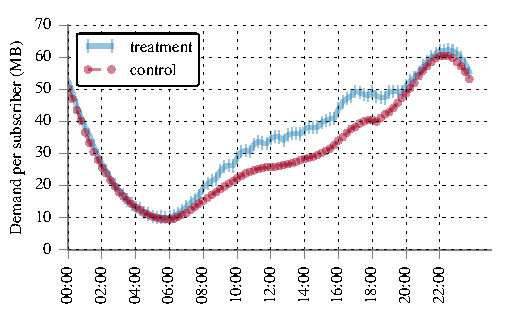
\includegraphics[width=\linewidth]{figures/weekday_demand_mean.pdf}
               \caption{Weekday traffic demand\label{fig:weekday-daily-usage}}
\end{subfigure}
%
\begin{subfigure}[b]{.99\linewidth}
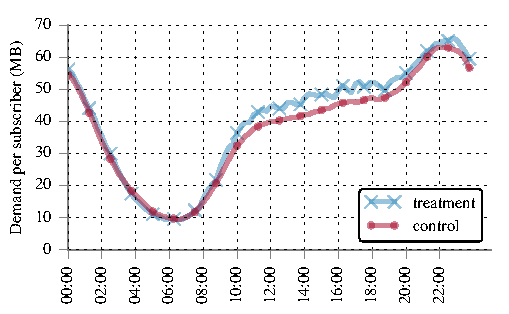
\includegraphics[width=\linewidth]{figures/weekend_demand_mean.pdf}
               \caption{Weekend traffic demand\label{fig:weekend-daily-usage}}
\end{subfigure}
%
\end{minipage}
\caption{Average subscriber demand (bytes every 15-minutes)}
\label{fig:traffic-demand-timeseries}
\end{figure}

Figure \ref{fig:traffic-demand-timeseries} shows the downlink traffic demand (bytes)
of an average subscriber over a 15-minute measurement period in a week.
We observe that subscriber behavior differs
significantly on weekdays and weekends. On weekdays, traffic demand 
increases monotonically from morning until prime-time in the evening. On 
weekends, there is a sharp rise in demand in the early morning period. Then, the
demand plateaus until the next sharp rise during the evening prime-time hours.
Previous reports indicate that the aggregate traffic volume for US fixed access
link providers usually troughs during mid-afternoon hours (between 2:00 PM -- 6:00 PM)
~\cite{sandvine20141h}. We do not observe such a trough in the subscriber 
demand in our dataset.

\begin{figure}[t]
\begin{minipage}{1\linewidth}
\centering
%
\begin{subfigure}[b]{1\linewidth}
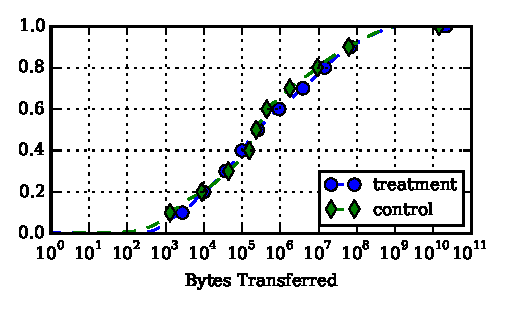
\includegraphics[width=\linewidth]{figures/cdf-all-bytes.pdf}
               \caption{Overall traffic demand for all subscribers at all times\label{fig:CDF-data-rate}}
\end{subfigure}
% maybe should be mean per day?
%
\begin{subfigure}[b]{1\linewidth}
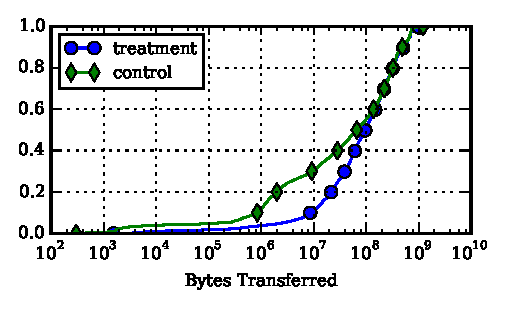
\includegraphics[width=\linewidth]{figures/cdf-per-device-perc95.pdf}
               \caption{Peak (95\%) traffic demand per subscriber\label{fig:CDF-data-rate-perc95}}
\end{subfigure}
%
\end{minipage}
\caption{Traffic demand (bytes every 15-minutes) for \control{} and \treatment{}\label{fig:traffic-demand-cdf}}
\end{figure}

Figure \ref{fig:CDF-data-rate} shows the distribution of the
all bytes transferred in the \treatment{} and \control{} set
over the three months of the dataset. Figure \ref{fig:CDF-data-rate-perc95}
plots the distribution of the peak (95th percentile) demand of the
subscriber over the three months of the dataset. The highest peak
demand achieved by subscribers in the \control{} and \treatment{}
groups were 10 GB in 15-mins. The median peak demand was 80 MB and
100 MB respectively.

We observe that although the overall series are similar, the peak demand of subscribers
is higher in the \treatment{} set. We expected the largest difference
in demands would be in the subscribers who have the heaviest demand already.
But unexpectedly, the lowest demanding 50\% of the subscribers in
\treatment{} have a much higher demand than the lowest demanding 50\% of \control{}.
We confirm that the both groups have similar median demands over each day. However
the daily peak demand is higher for the lowest demanding subscribers in
 \treatment{}, as compared to the lowest demanding subscribers in \control{}.

\begin{figure}[t]
\centering
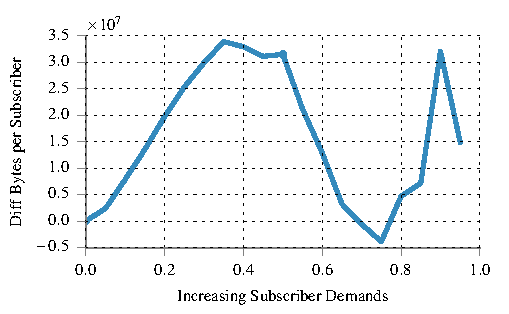
\includegraphics[width=\linewidth]{figures/diff_perc95_bytes_subsc-overall.pdf}
               \caption{Difference between \treatment{} and \control{}
               in peak (95\%) traffic demand\label{fig:diff-perc95}}
\end{figure}

We plot the distribution of the difference in peak subscriber demands for
the lowest to highest demanding subscribers in both groups (Figure~\ref{fig:diff-perc95}).
We see that the peak demand for the lowest demanding 70\% of the households of
the \treatment{} group is higher than the peak demand of the lowest demanding bottom-most
70\% of the \control{} group. These subscribers have a peak demand less than 200 MB.
For 20\% of the subscribers in the \control{} group with peak demands between 10 -- 70 MB,
the equivalent 20\% of the \treatment{} group has peak demands increased by 30 MB.

Under 15\% of subscribers in the \treatment{} group with peak demands more than 200 MB 
peak demands similar, or lower than the equivalent 15\% of subscribers in the \control{}
group, that has a lower capacity. The highest demanding subscribers in the \treatment{}
(beyond 800 MB peak demand) have demands 15 -- 30 MB more than the equivalent 15\% of 
the \control{} group. For the upstream, the \treatment{} group consistently has
a 2 MB higher peak traffic demand every 15 minutes as compared to the \control{} group
(except for the top 10\% users in the \treatment{} set who had a higher peak).

\begin{figure}[t]
\centering
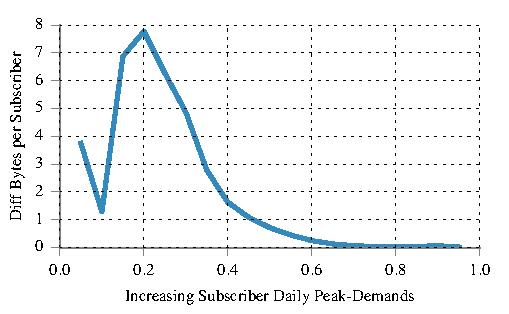
\includegraphics[width=\linewidth]{figures/diff_perc95_bytes_subsc-daily-normalized.pdf}
               \caption{Ratio of the difference between \treatment{} and \control{}
               in the daily peak traffic demand to the daily peak of the \control\label{fig:daily-ratio-perc95}}
\end{figure}

On investigating further, we observed that a similar percentage of 
subscribers with low peak demand in \control{} had a higher peak demand in \treatment{}.
40\% of the subscribers with lowest daily peak demands in the \treatment{} still
had more than double the traffic demand of the equivalent 40\% in the \control{} group.
(see Figure~\ref{fig:daily-ratio-perc95})

the 
There is negligible change in the daily peak 
demand for users who have high demands, and a large increase for users with a low demand.
Furthermore, we observe this affect is also present in the uplink.
There could be many reasons for this increase in demand, such as short
term activities (short videos or web browsing) 
that have a slightly higher traffic demand. Studying the applications 
responsible for such behavioral changes in traffic demand is out of the
scope of this paper and we leave it to future work.
\subsection{Prime-Time Ratio} \label{subsec:primetime}

The daily diurnal nature of Internet traffic demand requires that ISP providers 
design networks capable of handling load at the times when heaviest usage is 
observed. Such heavy demand is usually observed during prime time hours in the 
evening, when many subscribers heavily consume real-time entertainment traffic
(video) (seen as primarily responsible for high usage during these hours). The FCC defines 
Prime-Time as the local time from 7:00 PM to 11:00 PM.
\cite{fcc2014measuring-broadband}. To measure the concentration of network usage
during prime-time, we use Sandvine's definition of the \emph{Prime-Time 
ratio}: the ratio of the average traffic demand during prime-time hours to the average 
traffic demand in non-prime-time hours.\cite{sandvine20141h, sandvine20142h}.

We measure the prime-time ratio of the \control{} and \treatment{} group
for each contiguous four hour period in our datasets to find the evening hours with
the largest prime-time ratio. We observed that in our dataset,
the prime time ratio consistently peaks at 8:00 PM -- 12:00 AM for both
datasets.

%\begin{figure}[t]
%\begin{minipage}{1\linewidth}
%\centering
%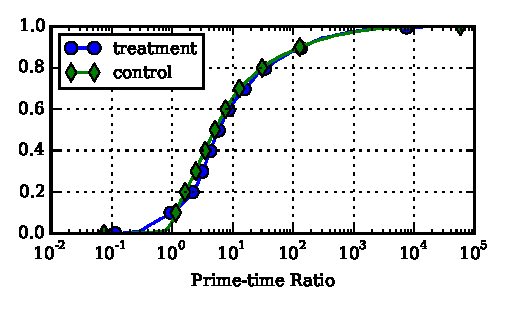
\includegraphics[width=1\linewidth]{figures/prime-time-ratio-per-device-cdf-MEAN.pdf}
%\caption{Prime-Time Ratio\label{fig:cdf-prime-time-ratio}}
%\end{minipage}
%\end{figure}

%\begin{subfigure}[]{.32\linewidth}
%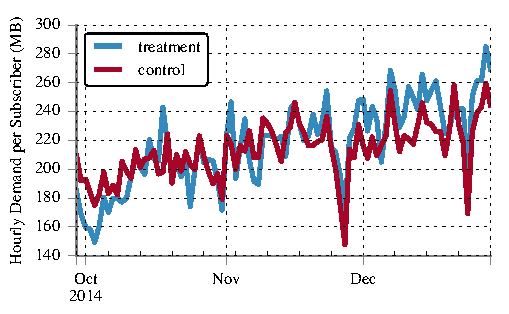
\includegraphics[width=1\linewidth]{figures/primetime_usage_per_day_per_subs.pdf}
%\caption{\label{fig:pt}}
%\end{subfigure}

%\begin{subfigure}[b]{.32\linewidth}
%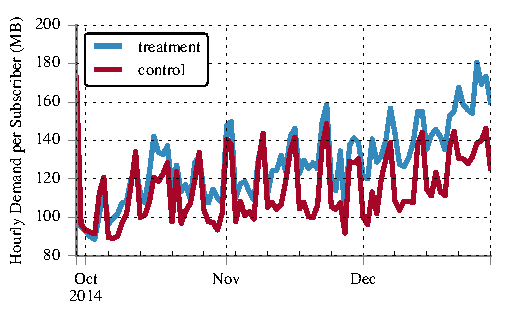
\includegraphics[width=1\linewidth]{figures/nonprimetime_usage_per_day_per_subs.pdf}
%\caption{\label{fig:non-pt}}
%\end{subfigure}


We observed that the hourly downlink traffic per 1000 subscribers between 8:00 PM -- 12:00 AM is 
209.5 GB for \treatment{}, and 205.1 GB for \control{}. However, during an average hour
outside of prime time, the traffic per 1000 subscribers is 122.3 GB for the higher tier
and 108.5 GB for the lower tier. This difference in demand during hours outside of the
daily prime-time is also apparant from the weekly usage patterns in Figure~\ref{fig:traffic-demand-timeseries}.

\begin{table}[t]
\begin{tabular}{| cc | c |c | }\hline
  &                    & Weekday         & Weekends \\\hline
\multirow{2}{*}{\begin{tabular}[c]{@{}l@{}}Hourly Traffic in\\ Prime-Time\end{tabular}}
& treatment          & 233.12          & 246.93   \\
& control            & 225.40          & 238.15   \\\hline
\multirow{2}{*}{\begin{tabular}[c]{@{}l@{}}Hourly Traffic in\\ Non-Prime-Time\end{tabular}}
& treatment & 124.18 & 143.08    \\
& control   & 104.30  & 133.16  \\\hline
\multirow{2}{*}{\begin{tabular}[c]{@{}l@{}}Prime-Time Ratio\end{tabular}}
& treatment & \textbf{1.88} &  1.73 \\
& control  &  \textbf{2.16} &  1.79 \\\hline
\end{tabular}
\caption{Hourly Traffic Demand during in prime-time hours (MB)\label{prime-time-demand}}
\end{table}


We calculate the prime-time ratio per day for the 
datasets groups over weekends and weekdays, as shown in Table \ref{prime-time-demand}.
%in figure~\ref{fig:cdf-prime-time-ratio}. A comparison shows 
On weekends, the prime-time ratios for both groups are
1.73 and 1.79 respectively. On the weekdays, the prime-time ratio for \control{}
is much higher, 2.16, as compared to treatment, 1.88. The demand
during prime-time hours on the weekdays for \treatment{} is within 4\% of
the \control{} traffic, thus there is no substantial
change. In contrast, the demand in non-prime-time hours (outside 8:00 PM -- 12:00 PM)
is much higher in the \treatment{} group, especially on weekdays. 

By definitition, the prime-time ratio is measured using total traffic volume in a day.
For our dataset, the prime-time ratio for the \treatment and \control groups
were 1.70 and 1.93 respectively. However, not all subscribers contribute equally
to the traffic volume. We observed that the median prime-time ratio \emph{per subscriber}
is 3.39 for the \treatment{} group and 2.91 for the \control{} group. This indicates
that demand during prime-time per subscriber has increased, but the total
traffic volume during non-prime-time hours has also increased substantially. For
subscribers that have a larger aggregate demand during non-prime-time hours, the prime
time ratio will be less than one. We found 9\% of the \control{} group and 14\% of 
the treatment group showed this behavior. These subscribers may be small home-run businesses,
users who work at home, or just users who have unexpected usage behaviors. 6\% of the 
subscribers in both groups had a prime-time ratio over 100.

Thus the overall demand of subscribers in the \treatment{} may have decreased by 
total volume of traffic, however, it has increased on a per-subscriber basis.
This result indicates that individual subscribers that do not contribute substantially
to the traffic volume are the ones who have higher usage in prime-time as compared to their
lower tier counterparts.

%Latency and performance 
%are adversely affected during prime-time, causing bottlenecks at home, the last 
%mile, in
%transit, or at the content server. For example, the Sandvine Global
%Internet Phenomena Report \footnote{The Sandvine Reports ~\cite{sandvine20141h,
%sandvine20142h}are released bi-annually and
%contain a detailed analysis of aggregate Internet usage. They are also referred
%to in the FCC reports~\cite{fcc2015progress-report, fcc2014measuring-broadband,
%fcc2014progress-report}} showed that devices in the same household selected  
%Netflix's own CDN (OpenConnect) during off-peak hours, and third party CDNs 
%(with differing
%performance) during prime-time. This may happen because Netflix OpenConnect is
%over-utilized during prime time~\cite{sandvine20141h}.
\subsection{Interpreting Utilization}
\label{subsec:utilization}

The prime-time ratio showed that there is a possible change in behavior of the \test due to an increase in capacity from 105 Mbps to 250 Mbps. Now, we try to answer the question: \emph{Is there any change in user behavior due to the upgrade, and if so, where?}
% the average user pattern from first subsection should also show the hours when avg usage is different => intuition for prime time and peak ratio.

\begin{figure}[ht!]
\centering
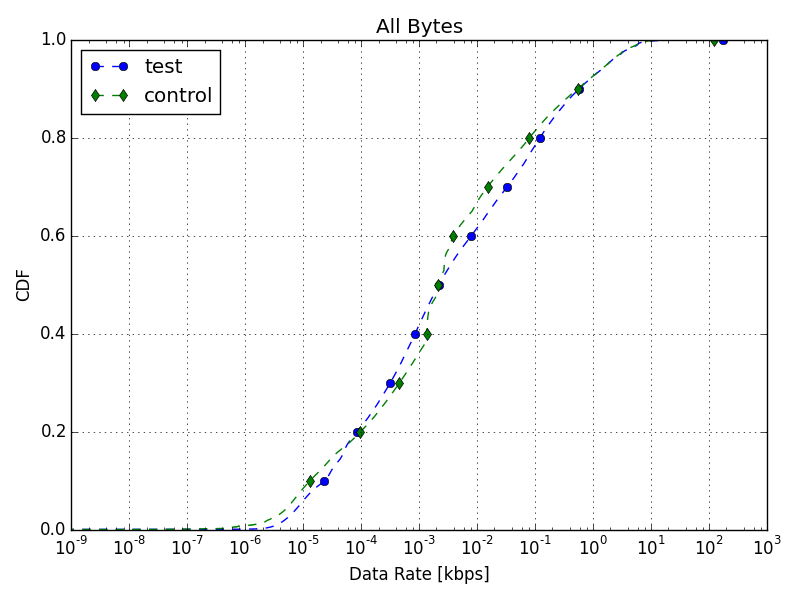
\includegraphics[width=0.90\linewidth]{figures/cdf-all-bytes.png}
  \caption{CDF of data rate per time slot for all devices (agg view of data): Overall not much change due to capacity increase. Median data rate ~ 2bps for 3 months x thousands of devices!}
  %http://sites.noise.gatech.edu/~sarthak/files/comcast/plots/full_dw/cdf-all-bytes.png
  \label{fig:CDF-data-rate-all}
\end{figure}

We thus investigate the distribution of the average data rate (a measure of data sent per time slot) for both sets. Figure ~\ref{fig:CDF-data-rate-all} shows that the the \control and \test set have a very similar usage behavior overall characterizing the bytes transferred throughout the day. Figure ~\ref{fig:TS-data-rate-daily} shows that the peak hour behavior of both sets is very similar, but during the day, the median data rate of \test set devices is slightly higher \todo{quantify} than the \control set.

%%%%%%%%%%%%%%%%%%%%%%%%%%%%%%%%%%%%%%%%%%%%%%%%%%%%%%%%%%%%%%%%%%%%%
\begin{figure}[ht!]
%\hspace*{-0.2in}
\begin{minipage}{0.90\linewidth}
\centering
%
%\hfill
\begin{subfigure}[b]{0.90\linewidth}
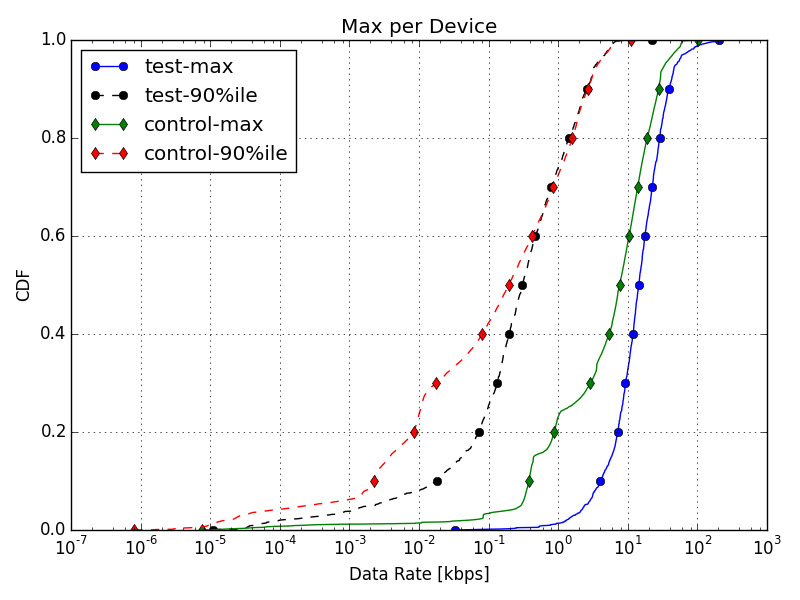
\includegraphics[width=\linewidth]{figures/cdf-max-per-device.png}
  \caption{CDF of max per device: test set has higher (max) average data rate below 10 kbps.  30\% of devices in the control set have a max data rate of 2 kbps while 30\% of test set has a max data rate of 10 kbps. (sanity check numbers, redo plot)}
  %http://sites.noise.gatech.edu/~sarthak/files/comcast/plots/full_dw/cdf-max-per-device.png
  \label{fig:CDF-data-rate-max}
\end{subfigure}
%
\vspace{-1em}
%
\begin{subfigure}[b]{0.90\linewidth}
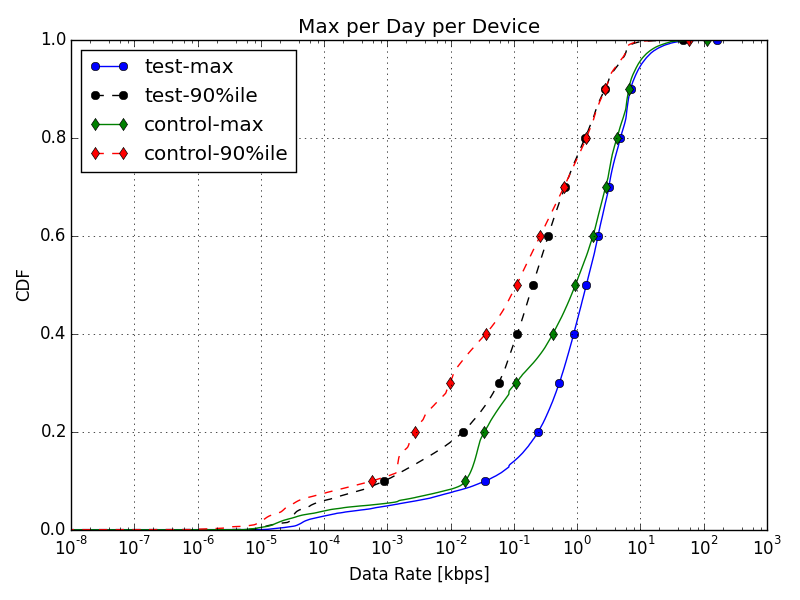
\includegraphics[width=\linewidth]{figures/cdf-max-per-day-per-device.png}
  \caption{CDF of max per device daily}
  \vspace{1em}
  %http://sites.noise.gatech.edu/~sarthak/files/comcast/plots/full_dw/cdf-max-per-day-per-device.png
  \label{fig:CDF-data-rate-max-daily}
\end{subfigure}
%\hfill
\end{minipage}
\caption{Peak Utilization: The maximum data rate varies for test and control set for low data rates, and this variation is present daily.}
\label{fig:peak-utilization}
% created using docs/metadata-separated.log
\end{figure}
%%%%%%%%%%%%%%%%%%%%%%%%%%%%%%%%%%%%%%%%%%%%%%%%%%%%%%%%%%%%%%%%%%%%%

Next we investigate the distribution of maximum data rate achieved by each household (figure~\ref{fig:CDF-data-rate-max}) over the three month period. Our results show that although the high utilizing households ($>$ 90\%-ile data rate) were similar throughout the set, showing no significant change in the maximum data rate, about 20\%-ile of the \test set devices saw a slight increase in the maximum data rate, which was much lower than link capacities. 
%the capacity utilization of both sets was similar during time slots with
% large data transfers, there is a certain difference in the maximum data
%rate per device for lower data rates \todo{needs a better more intuitive explanation}.

To confirm this, we plot the maximum data rate achieved \emph{daily} by each household (figure ~\ref{fig:CDF-data-rate-max-daily}). This showed that the maximum data rate achieved daily by low usage devices was higher for the \test set than the control set. We believe that this is an unbiased way to confirm the correlation between usage and capacity as the users did not know of the increased capacity, nor did they require it. The user's behavior does change when offered a higher capacity link, even though the overall capacity utilization stops increasing after a certain upper limit

We explore the reasons for such behavior: Discounting the possibility of this being a baseline behavior (i.e., \test set would show this even if it had the same capacity), we speculate that there could be two possible reasons for such a behavioral change: (1) short term downloads and usage achieves a slightly better data rate on a small time scale, or (2) real-time video quality is slightly higher, but not enough to completely saturate the access link capacity. Unfortunately, we miss these events due to a higher granularity of viewing data transferred only after 15 minutes.

%This agrees with the FCC's opinion that if given the option, users will
%adopt a higher tier bandwidth, even though they do not saturate the capacity~\cite{}.
%This also motivates the FCC to study deployment and adoption differently.
% Users may not adopt a higher bandwidth connection as they 
\paragraph{Different Perspectives of Utilization: }We take this opportunity to reflect on the issue of increasing broadband availability, deployment, and adoption being faced by the FCC~\cite{fcc2015progress-report}. The network usage increases slightly for low link utilization, without the user actively changing his/her behavior to saturate the link capacity.

The user, and therefore the FCC (representing the users' rights and demands), and the ISPs, are both correct, but have a different perspective of broadband utilization and adoption; the slight change in behavior for low utilization could motivate a user to adopt a higher bandwidth tier. From the ISP perspective though, the users link capacity utilization does not show any change due to the upgrade in connectivity and is therefore a deterrent to offering the higher tier.

Vice versa, an ISP may tell the user that they need to upgrade their broadband access link to achieve higher data rate for low throughput periods too. And the user might not need it, as their link capacity is clearly not saturated. \todo{... doesn't make sense yet something missing ...}

% some conclusion
We recommend that the FCC add multiple benchmarks, including \sg{ ... what comes here?}
\subsection{User Taxonomy based on Peak Ratio}
\label{subsec:peakratio}
% the ratio of the 90\%-ile to the median throughput per day.

\begin{figure}[ht!]
\begin{minipage}{0.90\linewidth}
\centering
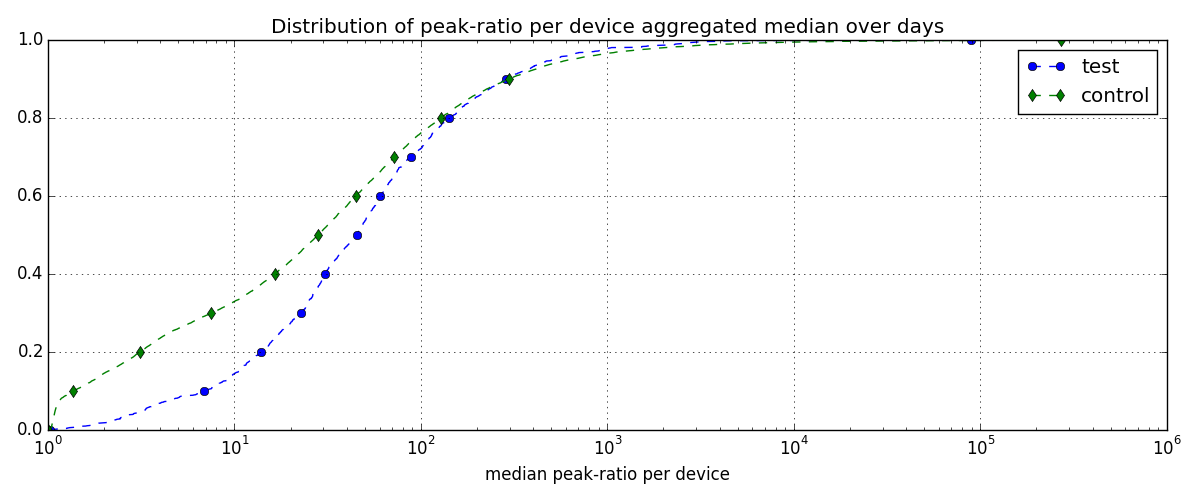
\includegraphics[width=1\linewidth]{figures/peakratio-CDF-devices-MEDIAN.png}
\caption{Median peak ratio per device showing that test set has higher daily ratio (50 times by median). Thus ISPs should condition their networks to 50 times the median usage for each user added in the worst case scenario.}
%http://sites.noise.gatech.edu/~sarthak/files/comcast/plots/full_dw/peakratio-CDF-devices-MEDIAN.png
\label{fig:CDF-peak-ratio-median}
\end{minipage}
\end{figure}

\paragraph{Peak Ratio: }To further characterize and compare the deviation of data rate for the \control and \test set, we examine \emph{peak-ratio} as defined in ~\ref{sec:methodology} 
Figure ~\ref{fig:CDF-peak-ratio-median} shows that the median peak-ratio for each device in the \test set is much larger than that of the \control set.
\todo{replace much larger with the exact number or percentage}.
\sg{Taken together} with our observations of a lower prime-time ratio of the \test set (section~\ref{subsec:primetime}) this implies that there are households in the \test set that achieve a peak-ratio $>$ 1, but not during the prime-time hour. We believe that these households might actually be small businesses or work-at-home users that peak during daytime hours instead of evening hours.

\begin{figure}[ht!]
\begin{minipage}{0.9\linewidth}
\centering
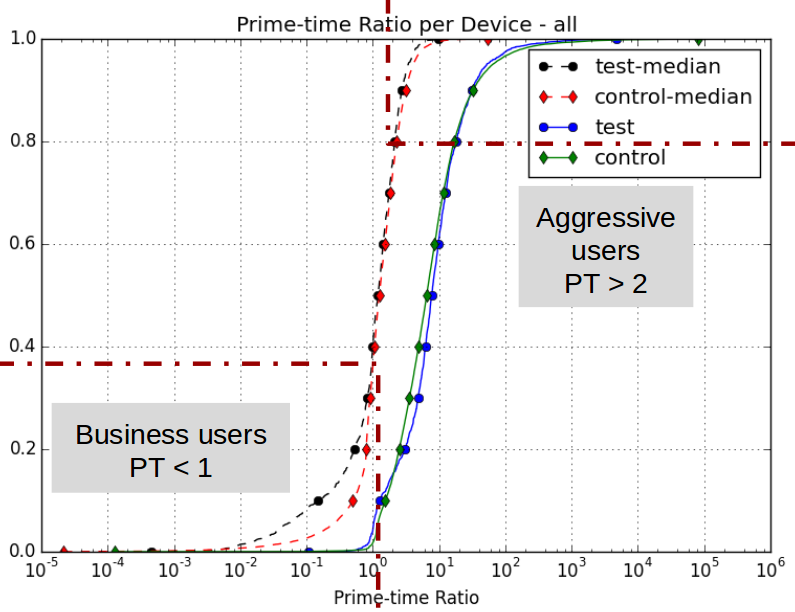
\includegraphics[width=0.9\linewidth]{figures/cdf-prime-time-ratio[replace].png}
\caption{(old) Prime Time ratio + usage can be used to divide users into four sets: aggressive all time + non aggressive all time, aggressive peak time, aggressive non-peak time (business hours). 30\% PT $<$ 1: possibly businesses with normal work-hours . 20\% PT $>$ 2: aggressive prime-time streamers}
%http://riverside.noise.gatech.edu:8083/separated/full/cdf-prime-time-ratio-per-device.png\\
%http://riverside.noise.gatech.edu:8083/plots/full_dw/prime-time-ratio-per-device-cdf-ALL.png
\label{fig:CDF-prime-time-ratio}
\end{minipage}
\end{figure}

The median peak-ratio per device itself shows a large range, from 1 to 10e6 (figure~\ref{fig:CDF-peak-ratio-median}), and the maximum peak-ratio per device was an order higher. Clearly there are some households that have a very even usage throughout the day (low peak ratio), and others that are extremely aggressive only at certain times (high peak ratio). We plot this segregation in figure ~\ref{fig:CDF-prime-time-ratio}.

\todo{EVERYTHING BELOW THIS IS TODO AND TODISCUSS}

\paragraph{User Taxonomy:} The Sandvine reports present a taxonomy of users based on their contribution to real-time entertainment traffic. We incorporate a similar definition based on contribution to data traffic, along with our observations of utilization, to present a taxonomy of the users in our dataset. One category of users is the non-utilizers, i.e., non-aggressive low bandwidth users, that contribute less than SOME THRESHOLD PERCENTILE to the daily data transferred \sg{these the ISP can ignore, also they probably don't need this tier as their utilization from the previous section must be super low}. The second category is of users contributing most aggressively to the data at the ISP \sg{these users will probably gobble up a higher capacity link if given a chance - they're the ones who effect all our graphs.. Need to check this claim}. We further subdivide this high utilizing subcategory based on differing prime-time ratio and peak-ratios follows... \todo{need to think and analyze this further: technical definition to do the analysis}
\begin{itemize}
\item Aggressive All-Time: Users having a low peak-ratio due to a lower variance. Is also expected to have a low prime-time ratio.
\item Aggressive Prime-Time: The usual streamer with a high prime-time ratio and a high peak ratio.
\item Aggressive Non-Prime-Time: Possibly a business user with a low prime-time ratio  but a high peak ratio
\end{itemize}

% other results:
%big difference (2 x median ratio) in per device per day ratios of 90%ile:median.
%weird shape again for values < ratio 100
%big difference in this ratio per day, and it is consistent across all individual sets + months.
%very large for Dec, slightly smaller for Nov
%interestingly, at higher ratios control is slightly > test. This means that certain devices in control set have a huge std (ratio) in a day as compared to test set which has a lower “max” ratio.

\todo{ TO PLOT :}
\begin{itemize}
\itemsep0em
\item peak ratio cdf vs no of devices
\item peak ratio cdf vs time of day where peak occurred
\item no of devices cdf vs time of day where peak occurred
\end{itemize}

Based on differing usage profiles within the same high tier bandwidth, we suggest that the FCC adopt multiple benchmarks based on usage characteristics to better characterize broadband availability, deployment, and adoption in the US. Such multiple benchmarks can be the minimum broadband speed required per user based on the kind of traffic expected during a day. ISPs can also offer these users better plans based on hour-of-the-day or usage caps to encourage more off-peak usage. These users probably don't cause latency spikes in PT.


We recommend multiple standards...
%\subsection{Traffic Asymmetry}
\label{subsec:asymmetry}

\begin{itemize}
\itemsep0em 
\item \todo{maybe this doesn't need a separate section, just comment on asymmetry in each of the above}
\item Cisco vs Alcatel: upload is increasing vs there's still too much download
\item Claim that its reducing due to uploads, but content is mostly download. Is the ratio still 10:1 (FCC thinks its ~25:3)
\item Compare with Sandvine asymmetry stats
\item Talk about 3 Mbps comparison with observed uplink in control and test set
\end{itemize}

\section{Discussion}
\label{sec:discussion}

\begin{itemize}
\itemsep0em
\item a better way to measure and offer broadband based on utilization?
\item multiple benchmarks of users segregated by usage
\item fcc measures: availability to deployment to adoption, maybe go the other way
\item survey sad adoption is low coz (1) user don't need bb and (2) its too expensive
\item if we can estimate (1) as false, providers can be encouraged to build and automatically
reduce (2)
\item significant section of 100 Mbps set shows that they do not cap usage per day in 15 min
\item this means low investment for next tier
\item but a set like 25 or 50 might show otherwise [need data]
\item other metrics: latency, etc considered by fcc
\end{itemize}
\section{Background and Related Work}\label{sec:related}

Traditionally, broadband performance analysis has attracted the attention of 
the measurement community. However with increasing availability of high 
bandwidth Internet services and FCC's recent interest in exploring traffic 
demand as a broadband benchmark \cite{fcc2015progress-report}, the focus has 
moved to evaluating the complex interplay between broadband demand and 
availability.
% basically availability includes performance, price, usage caps, etc. etc.

Our work build upon earlier analysis of the relationship between traffic demand 
and service capacity by Bischof \ea \cite{dasu-imc2014}. In this prior work, 
natural experiments were used hypothesize and infer causal relationships between 
the traffic demand\footnote{referred to as user demand, or usage in their work} 
and factors such as service capacity, performance, and price. They showed 
that demand increases with capacity, but ``follows a law of diminishing  
returns'', \ie increases in capacity for an already high tier causes a lower 
increase in demand, than if the upgrade would have occurred for a lower tier. 
Our work complements their study via a large-scale controlled experiment and 
examines in particular a high service tier (105 Mbps) that has not been studied 
before. Our dataset mitigates the affect of price, performance, and other 
potential biases (such as regional \cite{dasu-weather, dasu-region}, capped 
usage \cite{usage-caps}, and ``geek-effect'' \cite{dasu-imc2014}) by limiting 
the dataset to a large number of users selected randomly from the same service 
tier and location.

Zheleva \ea present a case study of the affect of an Internet service 
upgrade, from 256 kbps satellite to 2 Mbps terrestrial wireless, in rural 
Zambia. 
This work observed that the stark change in traffic demand three months after 
the upgrade caused a performance bottleneck. Our work focuses on higher 
service tier subscribers, who are presumably not bottlenecked, and studies 
changes in traffic demand without informing users of the upgrade.

Other efforts such as \cite{imc102-maier} study the characteristics of 
residential DSL broadband, and report the contributions of the most popular 
web applications to the total usage.
%They also note that most DSL users do not utilize their service capacity.
The bi-annual Sandvine reports \cite{sandvine2014report1h, 
sandvine2014report2h} provide an overview of overall Internet traffic 
demand from fixed lines and mobile carriers as well as an updated analysis of 
the most popular Internet applications. They showed that video accounts for 63\%
of traffic usage overall, and traffic demand peaks during the peak evening 
hours, possibly due to increasing video content consumption. Our work does not 
concern with the applications responsible for most traffic, but only with the 
peak period during which an individual subscriber's traffic demand is high.

%DASU: Other efforts have explored additional factors that may influence 
%service demand, including the weather [6], service capacity [36] and
%the type of region [8].

\label{lastpage}
\end{sloppypar}

%\appendix
%\input{appendix_sources}

%\vspace{-0.1in}
%\section*{Acknowledgments}


%% Bibliography
\pagebreak
\setlength{\bibsep}{0pt}
\small
\bibliographystyle{abbrv}
\flushleft\balance\bibliography{paper} 	% sigproc.bib is the name of the
										% Bibliography in this case 
%\bibliographystyle{abbrvnat_noaddr} % SPACE
%\theendnotes % ENDNOTES
}{% !onlyAbstract
}
%\section*{Appendices: FCC Issues of Inquiry}
\label{sec:appendix}

In the FCC report No. 14-113, released on Aug 5, 2014~\cite{fcc2014progress-report},
the Commission asks some relevant questions about broadband usage, and requests comments
from the community to improve its decision making process. The FCC report No. 15-10A1
answers some of these questions but raises issues for future progress reports.
We summarize their comments and questions with regards to usage behavior
as follows:
%\footnote{Note that the paragraph
%\# corresponds to the paragraph in the Eleventh Broadband Progress Report, FCC No. 
%15-10A1~\cite{fcc2015progress-report}\label{foot:fcc-issue-numbers}}

% comments for FCC:
% Can be mitigated by asking for usage instead from ISP first hop per household byte counters every 15 min. At least estimate usage (even if many apps in parallel) do they bottleneck or no?
% Why our comments are important:
%- measurement: understand the need for reco committee.
%- not biased (ATnT, verizon etc).
%- also understand broadband dynamics
%- important issues deserving our timely attention

\renewcommand{\thesubsection}{\Alph{subsection}}

\subsection{Tenth Broadband Progress Report}
\label{subsec:fcc2014}

Issues from the Tenth Broadband Progress Notice of Inquiry FCC 14-113, released 
August 5, 2014~\cite{fcc2014progress-report}

% purpose
\paragraph{3. Purpose of the Report. } We seek comment on the benchmarks we should use 
to define ``advanced telecommunications capability,'' explore whether we should establish 
separate benchmarks for fixed and mobile services, which data we should rely on in 
measuring broadband, whether and how we should take into account differences in 
broadband deployment, particularly between urban areas versus non-urban and Tribal 
areas, and other issues.
%We seek comment on whether we should modify the 4 megabits per second (Mbps) download and 1 Mbps upload (4 Mbps/1 Mbps) speed benchmark we have relied on in the past reports. We also seek comment on whether we should consider latency and data usage allowances as additional core characteristics of advanced telecommunications capability.

% speed and uses
\paragraph{6. Broadband Speed Benchmark.} Does service with speeds of 4 Mbps/1 Mbps 
provide consumers the ability to originate and receive these services? ... We seek 
comment on whether we should continue to benchmark broadband based on actual speeds, 
rather than advertised speeds, to the extent the two are different.

% peak usage time
% Peak usage is defined as the average data consumed between 7:00 to 11:00 pm on weeknights. The FCC asks if evaluating peak time usage is an efficient metric, or if average usage over a day should be considered instead.
\paragraph{13. Relying Upon Peak Usage Time.}
We seek comment on whether we should assess bandwidth requirements for a typical household
during peak Internet usage periods, from 7 pm to 11 pm on weeknights.
We seek comment on the types of broadband uses that are common, often used simultaneously, 
within a household during peak periods, and the appropriate bandwidth that would be 
necessary to accommodate those uses, to the extent that we determine that it is 
reasonable under section 706(b) to consider multiple simultaneous uses of broadband. 
We also seek comment on whether it is reasonable under the statute to set a speed 
benchmark on the basis of ``peak usage time.'' Is peak usage time an efficient metric? 
Should we instead consider the average household usage over a 24-hour period or over 
some other time period, or in some other manner entirely? We recognize that every 
household is unique, and that the services each household member uses will vary. We 
seek comment on whether establishing a reasonable household usage scenario during 
peak periods will assist the Commission in identifying a benchmark that is a 
necessary component of ``advanced telecommunications capability.''

% upload and download speeds needed at peak periods
\paragraph{15. Evaluating Downstream Usage during Peak Time.}
We seek comment on whether a download speed of 10 Mbps would adequately reflect
Congress’s goal of evaluating advanced telecommunications capability. Does 10 Mbps 
satisfy current demand, especially during peak time? Even assuming that it does, 
should the benchmark be higher than the minimum necessary to meet existing demand, 
i.e., should the benchmark be set to accommodate some level of anticipated future 
demand, particularly if the Commission does not intend to adjust the benchmark 
annually?... How should the Commission forecast future household broadband uses 
to justify such a benchmark?

\paragraph{17. Evaluating Upstream Usage.} We thus seek comment on whether a 1 Mbps 
upload speed is sufficient to meet the goals set forth in section 706. We also seek 
comment on whether there is a basis for the disparity between download and upload 
speeds in any speed threshold(s) used by the Commission. For example, if the Commission 
increases the download speed benchmark, should it also increase the upload speed benchmark?
Why or why not?

% Adoption based broadband benchmarking
\paragraph{18. Setting a Speed Benchmark Based on Adoption Rates.} We seek comment on 
whether the Commission should consider the rates at which consumers are adopting 
particular speeds when setting a speed benchmark. We seek comment on whether a higher 
benchmark is appropriate when the Fourth Measuring Broadband America Report indicates 
that consumers continue to migrate to higher broadband speeds.

% Taxonomy of users even in a single speed tier
\paragraph{19. Adoption of the Fastest Available Speed Tier} Should the benchmark be based 
on the fastest speed tier to which a substantial portion of
consumers subscribe? How should the Commission define ``substantial portion'' and how 
should we interpret such demand? Would using such a metric accurately reflect the market 
choices and needs of consumers based on the service offerings available to them? Does a 
particular adoption rate (to be determined) by consumers with access to broadband 
demonstrate that there is sufficient demand for that speed tier? Does adoption at a 
certain speed demonstrate or suggest that service of that speed is necessary to 
enable users to originate and receive high-quality voice, data, graphics, and video 
telecommunications?

% separate benchmarks: min broadband = 10/1, better broadband = 25/3, schools and libraries = 100...
%broadband requirements are not uniform throughout the nation. Some users will have significantly greater needs. The FCC is interested to know whether it should opt for multiple benchmarks depending on user scenario, usage, occupation, etc.? 
\paragraph{22. Multiple Speed Benchmarks.} We also seek comment on whether the Commission
should consider establishing multiple benchmarks. Multiple benchmarks could improve our ability
to assess whether advanced telecommunications capability is being deployed in a reasonable
and timely manner by recognizing that broadband requirements are not uniform throughout the 
nation. For example, while the ``typical use'' 10 Mbps download speed benchmark described 
above is intended to satisfy common household broadband demand, some users, such as larger 
families or teleworkers, will have significantly greater bandwidth needs. We seek comment 
on whether the Commission should adopt more than one speed benchmark and if so, how we 
should use the different benchmarks to evaluate whether deployment is occurring in a 
reasonable and timely manner.

% IMP: Usage as a Broadband Benchmark
\paragraph{27. Usage as a Broadband Benchmark.} The Commission has indicated that it might consider
data usage allowance as a core characteristic that affects what consumers can do with their broadband
service.
Should we include usage in our section 706 assessment? If so, how?
%We seek comment on what data usage allowances most broadband providers offer today, and the impact of these usage allowances on setting a benchmark. For example, do consumers routinely exceed the usage allowance for the service to which they subscribe and if so, is additional capacity available for an additional fee? If so, how frequently do consumers avail themselves of that option?

% how to measure the amount of data consumers use - form 477
\paragraph{29. Broadband Usage Threshold. } How would the Commission implement a broadband usage
threshold? Should the Commission focus on the amount of data that consumers actually use each month,
instead of what broadband providers typically offer? What information, reports, or other sources are
available to measure the amount of data consumers use monthly?
%In particular, are there any sources
%concerning usage that the Commission could use to assess which carriers meet or do not
%meet the usage threshold?

% How should deployment be measured
\paragraph{37. Improving Progress Reports. } We seek comment on ways to improve the Commission’s
annual broadband progress reports, such as incorporating new data sources or conducting our
analysis differently. Are there other ongoing efforts to collect broadband deployment or
availability data that were not available, or that we did not include, in prior reports? 
We seek input on whether there are any particular surveys or other reports that would be
particularly beneficial to our section 706 analysis.


\subsection{Eleventh Broadband Progress Report}
\label{subsec:fcc2015}

Issues from the Tenth Broadband Progress Report and Notice of Inquiry FCC 15-10A1,
released February 9, 2015~\cite{fcc2015progress-report}.

% why some people do not adopt broadband - motivation to study usage patterns
\paragraph{7. Impact of Broadband Adoption on Availability and Deployment.}
As part of our inquiry
into ``the availability of advanced telecommunications capability to all Americans,''
we also examine broadband adoption--some reasons why Americans choose not to adopt
broadband could reflect factors that are relevant to its ``availability,'' such as
price and quality. While we continue to see that adoption lags behind deployment
to a significant degree, at all speeds, we do not know precisely why.
%The recent 2014 NTIA Digital Nation Report found the top reason given for
%non-adoption was consumers simply not wanting broadband, and the second most
%cited reason was because it was too expensive.
%Americans with lower median incomes and where the poverty rate,
%rural population rate, and unemployment rate is higher tend to have lower
%broadband adoption rates. These facts raise questions about whether
%broadband is ``availab[le] . . . to all Americans'' as the statute requires,
%and we will continue to evaluate both how we can improve our analysis in future
%Reports and how the Commission can address the adoption gap.
Although we evaluate adoption separately from deployment and our determination
about whether broadband is being deployed in a reasonable and timely fashion stands
independently from our evaluation of broadband adoption, examining adoption is useful
both as an indicator of what Americans may consider to be needed and separately as
a stimulator for deployment.

% need to add usage patterns to this study
%\paragraph{10. }
%In addition, we expect to examine other factors of availability, including usage
%allowances and price, latency, whether service at the relevant speed is available
%on a consistent and reliable basis, and whether the network is secure. We expect
%to examine these factors in the next Inquiry and will seek out ways to improve our
%ability to evaluate them, relevant to both fixed and mobile services.

%deployment will occur only if people adopt and ISPs can make money off it => must study why all people don't adopt => study usage (bb not needed) vs price (bb too expensive).
%\paragraph{12. } As a consequence of our conclusion that advanced telecommunications
% capability is not being deployed to all Americans in a reasonable and timely fashion,
% section 706 mandates that the Commission ``take immediate action to accelerate
% deployment of such capability by removing barriers to infrastructure investment and
% by promoting competition in the telecommunications market.''

% multiple standards - why and why not
\paragraph{23. Multiple Benchmarks. } NCTA recommends that the Commission ``should use
multiple benchmarks
in performing its section 706 analysis rather than just one'' because doing so would ``better
reflect the multi-faceted nature of today’s broadband marketplace, which features a wide
variety of technologies and services that are able to cater to the varying needs of American
consumers.'' Others in the record disagree, stating, for example, that ``[t]here is
no substantive rationale provided to warrant having multiple standards. One standard sends
a clear and easily understood message to all parties.'' At this time we decline to use multiple 
benchmarks in this Report. We find that the single benchmark we use in this Report, which
relies on a higher speed benchmark than prior reports, is the appropriate means to allow us
to analyze whether advanced service is being deployed.

% speed factor
\paragraph{26. Redefined Speed Benchmark. } ... requires consumers to have access to actual
download (i.e., to the customer) speeds of at least 25 Mbps and actual upload (i.e., from 
the customer) speeds of at least 3 Mbps (25 Mbps/3 Mbps). For schools and classrooms, we use
the same benchmark that the Commission already established for schools and classrooms of a 
short term benchmark of 100 Mbps per 1,000 students and staff and a long-term speed 
benchmark of 1 Gbps per 1,000 students and staff.

% consumers adopt higher speeds when they have the option
\paragraph{41. Consumer Needs affect Broadband Adoption. } Our own assessment of
consumers’ likely needs is confirmed by examining broadband
adoption. When speeds of 25 Mbps/3 Mbps are available, a substantial 
and fast-growing number of consumers are adopting and migrating to 
higher speeds. Examining the adoption trends from December 2011 to 
December 2013, we find that the adoption rate of this service or 
higher quadrupled. Customers are deciding for themselves at a very 
rapid rate that they need services at this or higher speeds

% household level rather than user level granularity
\paragraph{47. Consider Broadband at the Household Level. }
Because consumers usually purchase fixed broadband service for the household, and because the 
deployment data represent households rather than individuals, we find it reasonable to consider 
broadband needs at a household level, rather than what each individual household member, individually, 
may need.

% why single benchmarks might not work - there are many types of users within the same tier
%\paragraph{52. }
%Some commenters urge us to retain the 4 Mbps/1 Mbps benchmark228 or increase the
%benchmark to 10 Mbps/1 Mbps. ATnT asserts that section 706(b) is not ``myopically'' focused on the 
%subset of consumers who are the heaviest users.230 We agree. Section 706(b) is not ``myopically'' 
%focused on any particular subset of consumers. But it does require the Commission to assess deployment 
%of advanced services that are capable of performing specific functions, and doing so at a high 
%quality.

% availability and deployment
%\paragraph{64. }
%We affirm the Commission’s prior findings that, for the purpose of our analysis, the 
%terms broadband ``deployment'' and ``availability'' are broader than mere physical 
%presence of broadband networks. This interpretation is the most natural reading of
%section 706(b). Moreover, section 706 requires the Commission to conduct an inquiry
%into broadband ``availability'' and determine whether broadband ``is being deployed''
%in a reasonable and timely fashion. The statute does not indicate that a determination
%about whether broadband is being deployed must consider a set of circumstances narrower
%than the ``availability'' inquiry. We continue to interpret ``all Americans'' as establishing
%the goal of universal broadband availability for every American. As such, our annual
%determination as to how broadband ‘‘is being deployed’’ is simply an assessment of how
%well we are progressing toward the goal of ``availability to all Americans.''

% Factors influencing adoption: availability, price, quality, ...
\paragraph{65. Assessing Availability and Deployment.} We conclude that in determining
whether broadband is ``being deployed to all Americans in a reasonable and timely fashion,''
we must look at a variety of factors that affect access to broadband. ... Accordingly, as
in prior Reports, our inquiry includes an assessment of a variety of factors indicative of
broadband availability, such as price, quality, and adoption by consumers, as well as
physical network deployment.

%VI. REMOVING BARRIERS & PROMOTING COMPETITION 141.
\paragraph{141. Removing Barriers to Promote Competition. }
%In light of our finding that advanced telecommunications capability is not being deployed to all Americans in a reasonable and timely manner, the Commission must ''take immediate action to accelerate deployment of such capability by removing barriers to infrastructure investment and by promoting competition in the telecommunications market.'' In the last two Reports, the Commission found numerous barriers to infrastructure investment. In particular, the high costs associated with deploying and operating a broadband network coupled with low broadband adoption rates, present barriers.
As we have done in the past, we will continue to work on removing barriers to infrastructure
investment by identifying and helping to reduce potential obstacles to deployment, 
competition, and adoption -- concepts that we continue to recognize are tightly linked.

%usage of broadband is a barrier to deployment of higher speeds.
% measure usage of areas with no deployment (open data) - if it seems aggressive for a certain percentage of total people in that are => cost price analysis to deploy bb there. (almost the same as comcast's requirement to get at least 10 signatures in rural areas)
\paragraph{142. Barriers to Deployment and Adoption. } Because providers will consider
adoption rates when determining whether to build out facilities and offer service 
a particular area, we consider barriers to adoption as well as deployment. The 
key barriers to deployment and adoption include: (1) costs and delays in building 
out networks; (2) broadband service quality; (3) lack of affordable broadband 
Internet access services; (4) lack of access to devices and other broadband-capable
equipment; and (5) barriers to entry by potential competitors and, consequently, 
lack of competitive choice for consumers.
%only way is to show provider that on aggregate the deployment will be revenue generating => usage patterns to show that lower tiers are not satisfactory
%but we can't do this with current data unless comcast gives us low tier data!

\end{document}

% Local Variables:
% TeX-command-default: "LaTeX PDF"
% End:

